 %% LaTeX Template for ISIT 2019
%%
%% by Stefan M. Moser, October 2017
%% 
%% derived from bare_conf.tex, V1.4a, 2014/09/17, by Michael Shell
%% for use with IEEEtran.cls version 1.8b or later
%%
%% Support sites for IEEEtran.cls:
%%
%% http://www.michaelshell.org/tex/ieeetran/
%% http://moser-isi.ethz.ch/manuals.html#eqlatex
%% http://www.ctan.org/tex-archive/macros/latex/contrib/IEEEtran/
%%

\documentclass[conference,letterpaper]{IEEEtran}

%% depending on your installation, you may wish to adjust the top margin:
\addtolength{\topmargin}{9mm}

%%%%%%
%% Packages:
%% Some useful packages (and compatibility issues with the IEEE format)
%% are pointed out at the very end of this template source file (they are https://www.overleaf.com/5925174675mmtrqctdffvj
%% taken verbatim out of bare_conf.tex by Michael Shell).
%
% *** Do not adjust lengths that control margins, column widths, etc. ***
% *** Do not use packages that alter fonts (such as pslatex).         ***
%
\usepackage[utf8]{inputenc} 
\usepackage[T1]{fontenc}
\usepackage{url}
\usepackage{ifthen}
\usepackage{cite}
\usepackage[cmex10]{amsmath} % Use the [cmex10] option to ensure complicance
                             % with IEEE Xplore (see bare_conf.tex)

%% Please note that the amsthm package must not be loaded with
%% IEEEtran.cls because IEEEtran provides its own versions of
%% theorems. Also note that IEEEXplore does not accepts submissions
%% with hyperlinks, i.e., hyperref cannot be used.
\usepackage{graphicx}

%% Macros
\def\trainingset{\{x_i,y_i\}_{i=1}^{N}}
\def\pNMLSingle{p_{\hat{\theta}(z^n,x,y)} (y|x)}

\interdisplaylinepenalty=2500 % As explained in bare_conf.tex


%%%%%%
% correct bad hyphenation here
\hyphenation{op-tical net-works semi-conduc-tor}

% ------------------------------------------------------------
\begin{document}
\title{A New Look at an Old Problem: A Universal Learning Approach to Linear Regression} 

%%% Several authors with up to three affiliations:
\author{%
  \IEEEauthorblockN{Koby Bibas}
  \IEEEauthorblockA{School of Electrical Engineering\\
                    Tel Aviv University\\
                    Email: kobybibas@gmail.com}
  \and
  \IEEEauthorblockN{Yaniv Fogel}
  \IEEEauthorblockA{School of Electrical Engineering\\
                    Tel Aviv University\\ 
                    Email: Yaniv.fogel8@gmail.com}
  \and
  \IEEEauthorblockN{Meir Feder}
  \IEEEauthorblockA{School of Electrical Engineering\\
                    Tel Aviv University\\ 
                    Email: meir@eng.tau.ac.il}
}


\maketitle

%%%%%%
%% Abstract: 
%% If your paper is eligible for the student paper award, please add
%% the comment "THIS PAPER IS ELIGIBLE FOR THE STUDENT PAPER
%% AWARD." as a first line in the abstract. 
%% For the final version of the accepted paper, please do not forget
%% to remove this comment!
%%
\begin{abstract}
%    THIS PAPER IS ELIGIBLE FOR THE STUDENT PAPER AWARD.
Linear regression is a classical paradigm in statistics. 
A new look at it is provided via the lens of universal learning.
In applying universal learning to linear regression the hypotheses class represents the label $y\in {\cal R}$ as a linear combination of the feature vector $x^T\theta$ where $x\in {\cal R}^M$, within a Gaussian error.
The Predictive Normalized Maximum Likelihood (pNML) solution for universal learning of individual data can be expressed analytically in this case, as well as its associated learnability measure. 
Interestingly, the situation where the number of parameters $M$ may even be larger than the number of training samples $N$ can be examined. 
As expected, in this case learnability cannot be attained in every situation; nevertheless, if the test vector resides mostly in a subspace spanned by the eigenvectors associated with the large eigenvalues of the empirical correlation matrix of the training data, linear regression can generalize despite the fact that it uses an ``over-parametrized'' model. 
We demonstrate the results with a simulation of fitting a polynomial to data with a possibly large polynomial degree.
\end{abstract}

%%%%%%%%%%%%%%%%%%%%%%%%%%%%%%%%%%%%%%%%%%%%%%%%%%%%%%%%%%%%%%%%%%%%%%%%%%%%%%%%

\section{Introduction} \label{Introduction}
Linear regression, using least squares, is probably one of the most standard techniques in statistics, \cite{lawson1995solving}. This work provides a new view of this problem based on recent results in universal learning. In particular, the common assumption in linear regression is that the number of training samples needs to be much higher than the number of features in order to be able to generalize \cite{james2013introduction}.
Recently, the success of Deep Neural Networks (DNNs) in which the number of learnable parameters is in several orders of magnitudes greater than the size of the feature space requires rethinking that assumption. 
The new view we provide will show that sometimes generalization can be attained even in the ``over-parameterized'' regime.

Before diving into this analysis, a short introduction to universal learning is provided. In the common situation of supervised machine learning, a training set is given consisting of $N$ pairs $z^N=\{(x_i, y_i)\}_{i=1}^{N}$, where $x \in {\cal X}$ is the data or the features and $y \in {\cal Y}$ is the label. Then, a new $x$ is given and the task is to predict its corresponding label $y$. 
In the information theoretic framework considered in a variety of works, e.g., \cite{universal_prediction} and more recently \cite{FogelFeder2018}, prediction is done by assigning a probability distribution $q(\cdot|x)$ to the unknown label, and the prediction loss is the log-loss:
\begin{equation}
\mathcal{L}(q;x,y) = -\log {q(y|x}).
\end{equation}
Clearly a reasonable goal is to find the predictor $q$ with the minimal loss for the test sample. However, this problem is ill-posed unless additional assumptions are made.

First, a ``model'' class, or `hypotheses'' class must be defined. 
This class is a set of conditional probability distributions
\begin{align} P_\Theta = \{ p_\theta(y|x),\;\;\theta\in\Theta\} \end{align} 
where $\Theta$ is a general index set. 
This is equivalent to saying that there is a set of stochastic functions  $\{ y=g_\theta(x),\;\;\theta\in\Theta\}$ used to explain the relation between $x$ and $y$.

Next, assumptions must be made on how the data and the labels are generated. 
In the stochastic setting, it is assumed that there is a true probabilistic relation between $x$ and $y$ given by an (unknown) model from the class $P_\Theta$. 
A more general setting, used in the variety of works in machine learning, is the Probably Approximately Correct (PAC) established in  \cite{valiant1984theory}. 
In PAC $x$ and $y$ are assumed to be generated by some source $P(x,y)=P(x)P(y|x)$, but unlike the standard stochastic setting $P(y|x)$ is not necessarily a member of the hypothesis class. 
In both the stochastic and PAC settings the goal is to perform as well as a learner that knows the true probability.

The most general setting, however, and the one used in this paper is 
the individual, where the data and labels of both the training and test are specific and individual.
In this setting the goal can no longer be to perform as well as a learner that knows the true probability. Instead, following \cite{universal_prediction}, the goal is to seek a learner that can compete with a ``genie'' or a reference learner that knows the desired label value, but is restricted to use a model from the given hypotheses class $P_\Theta$. In addition, as discussed in \cite{FogelFeder2018}, the reference has no knowledge which of the samples is the test. Thus, the reference chooses
\begin{align} \hat{\theta}(z^N,x,y)  = \arg\max_\theta \left[ p_\theta(y|x) \cdot\Pi_{i=1}^N p_\theta(y_i|x_i) \right] \end{align}
The log-loss difference between a universal learner $q$ and the reference is the regret:
\begin{equation} \label{eq:genie_regret}
R(z^N,x,y,q) = \log \frac{p_{\hat{\theta}(z^N,x,y)}(y|x)}{q_(y|x;z^N)}.
\end{equation}
% pNML
As advocated in \cite{FogelFeder2018}, the chosen universal learner solves:
\begin{equation} \label{eq:minmax_prob}
\min_q \max_y R(z^N,x,y,q) = R^*(z^N,x)
\end{equation}
Following \cite{shtar1987universal} this learner, called the Predictive Normalized Maximum Likelihood (pNML), is given by
\begin{equation} \label{eq:pNML}
q_{\mbox{\tiny{pNML}}}(y|x;z^N)=\frac{\pNMLSingle}{\sum_{y\in {\cal Y}} \pNMLSingle}.
\end{equation}
Note that this pNML probability assignment was essentially proposed earlier, see \cite{roos2008sequentially,roos2008bayesian}, with a different motivation as one of the possible variations of the Normalized Maximum Likelihood (NML) method of \cite{shtar1987universal} for universal prediction.

In order to obtain the pNML the following procedure is executed: assuming the label of the test data is known, find the best model that fits it with the training samples, and predict the assumed label by it. 
Repeat the process for all possible labels. 
Then, normalize to get a valid probability distribution which is the pNML learner.
The regret of the pNML, $R^*(z^N,x)$ is the logarithm of its normalization factor
\begin{equation} \label{eq:pNML_regret}
R^*(z^N,x) = \log \left\{ \sum_{y\in {\cal Y}} \pNMLSingle \right\}.
\end{equation}

In considering linear regression, $y\in {\cal R}$ is the scalar label, $x\in {\cal R}^M$ is the feature vector (sometimes the first component of $x$ is set to $1$ to formulate affine linear relation), and the model class is the set:
\begin{equation} \label{regression_model}
\left\{ p_{\theta}(y|x) 
=\frac{1}{\sqrt[]{2\pi\sigma^2}}\exp\left\{-\frac{1}{2\sigma^2}\big(y- x^T\theta \big)^2\right\}, \;\; \theta \in {\cal R}^M \right\} 
\end{equation}
That is, the label $y$ is a linear combination of the components of $x$, within a Gaussian noise. As shown below, in this case the pNML and its learnability measure can be evaluated explicitly.

% ERM
The pNML approach deviates from the standard Empirical Risk Minimization (ERM) \cite{vapnik1992principles} approach.
In ERM, given a training set and hypothesis class $\{p_\theta(y|x),\ \theta \in \Theta\}$, a learner that minimizes the loss over the training set is chosen:
\begin{equation}
q_{\mbox{\tiny{ERM}}}(y|x) = \underset{p_\theta}{\textit{argmin }} \frac{1}{N}\sum_{i=1}^{N}  \mathcal{L}(p_\theta; x_i, y_i).
\end{equation}
In the linear regression model (\ref{regression_model}), one chooses the least squares solution over the training set for the linear coefficients. 
This, however, may lead to large generalization log-loss error.

The paper has two main contributions.
First, it provides an explicit analytical solution for the pNML learner and its ``learnability'' measure (which is the minmax regret (\ref{eq:pNML_regret})) for the linear regression hypothesis class. This includes also the regularized case where the norm of the coefficients vector is constrained. Second, based on the analysis of the learnability measure, it is shown that even in the over-parameterized case where the number of parameters $M$ may be larger than the training size $N$, if the test data comes from a ``learnable space'' successful generalization occurs.
This phenomenon may explain why other over-parameterized models such as deep neural networks are successful for ``learnable'' data.

The paper outline is as follows.
Section \ref{sec:related_works} presents some related work. 
Section \ref{sec:formal_problem_def} provides the formal problem definition, while the pNML evaluation for the regression problem is given in sections \ref{sec:pNML_eval} and \ref{sec:pNMLwithReg}. 
In-depth analysis of the learnable space is given in section \ref{sec:learnable_space}. 
Simulation of the pNML and its regret for the problem of fitting a polynomial to data is described in section \ref{sec:simulation} and the conclusions are in section \ref{sec:conclusion}.

\section{Related Works} \label{sec:related_works}
In this section, we briefly mention related works on model generalization, least squares regression and the confidence of the least squares predictions.

\textbf{Model Generalization.} 
Understating the model generalization capabilities is considered a fundamental problem in machine learning  \cite{vapnik2013nature}. 
As noted, most of the theoretical work in learning use the PAC setting. In that setting, a common measure is the VC Dimension that can be used to upper bound on the test generalization error.
For DNNs, the VC dimension is linear with the number of parameters \cite{sontag1998vc}, yet the empirical evidence demonstrates that DNN's have state of the art generalization performance. This makes the VC dimension irrelevant for assessing the generalization error of DNNs.

\textbf{Least Squares.}
The least squares algorithm is widely used in linear regression due to its robust performance and simplicity of implementation.
In addition to the explicit formula for its solution, it can be solved sequentially, via the Recursive Least Squares (RLS) algorithm, which is an efficient online method for finding the linear predictor that minimizes the squared error over the training data \cite{hayes19969}.
In learning field, the least squares estimator is used for prediction in both ERM and Bayesian approaches \cite{fornalski2015applications}. 
This paper provides an analysis in the individual setting, in the realm of the pNML approach.

\textbf{Outliers detection and confidence.}
In order to evaluate a pointwise confidence measure for linear regression, several methods were proposed. 
Leverage values are employed to identify outliers with respect to their feature values \cite{cardinali2013observation}. 
A leverage value is a measure of the distance between an observation and the center of the data
\begin{equation}
h_{ii}=x_i^T(XX^T)x_i
\end{equation}
where $X$ is the correlation matrix of the training set and $x_i$ is the feature value which is examined.
If the leverage value $h_{ii}$ of observation is large, the observation is considered as an outlier.
Using the pNML, we fit a learner assuming the label of the test sample is known. 
Therefore, testing whether it is an outlier can produce prediction confidence.
In section \ref{sec:pNML_eval}, we get analytically similar expression to the leverage measure.

Another approach for finding the reliability of the prediction is to compose confidence intervals \cite{trevor2009elements}.
Confidence intervals are a pointwise measure that is sensitive to the variability of the features and sample size.
Denote $\hat{y}$ as the predicted value of $x$ and  $\hat{\sigma}^2$ as the empirical error of the prediction, under the assumption of stochastic i.i.d data and existence of white noise, a confidence interval convergences is distribution to
\begin{equation}
(\hat{y} - y) \xrightarrow{} \mathcal{N}(0, \hat{\sigma}^2 x^T(XX^T)^{-1}x)
\end{equation}


% ----------------------------------------------
% Linear Regression: Formal Problem Definition
% ----------------------------------------------
\section{Linear Regression: Formal Problem Definition} \label{sec:formal_problem_def}
Given N pairs of data and labels $\{x_i, y_i\}_{i=1}^{N}$ where $x_i \in R^M, y\in R$ are deterministic, the model takes the form:
\begin{equation}
\begin{split}
y_1&=x_1^T \theta + e_1 \\
   &\ \vdots \\
y_{N}&=x_{N}^T \theta + e_{N} \\
\end{split}
\end{equation}
where $\theta \in R^M$ are the learnable parameters and the $e_i \in R$ are zero mean, Gaussian, independent with variance of $\sigma^2$. 
The goal is to predict $y$ based on a new data sample $x$. 
Under the assumptions $y$, conditioned on $x$, has a normal distribution that depends on the learnable parameters $\theta$ 
\begin{equation}
p_{\theta}(y) 
=\frac{1}{\sqrt[]{2\pi\sigma^2}}\exp\left\{-\frac{1}{2\sigma^2}\big(y- x^T\theta \big)^2\right\}.
\end{equation}
The unknown parameter vector $\theta$ belongs to a set $\Theta$, which in the general case is the entire $R^M$. In the regularized version (that leads to Ridge regression \cite{ridgeregression}), $\Theta$ is the sphere $|\theta|\leq A$. 
In the next section, the pNML will be evaluated for this hypotheses class. 
Recall that the pNML learner of $y$ given the the test sample $x$ and the training set $z^N=\{(x_i,y_i)\}_{i=1}^{N}$ is given by:
\begin{equation} \label{eq:pNML_def}
q_{\mbox{\tiny{pNML}}}(y|x;z^N) = \frac{1}{K} p_{\hat{\theta}(z^N;x,y)}(y|x).
\end{equation}
where in the linear regression case 
\begin{align}
\hat{\theta}(z^N,x,y)= \arg\min_{\theta\in\Theta} \left[ \sum_{i=1}^N \left(y_i - x_i^T\theta \right)^2 + \left(y-x^T\theta\right)^2 \right]
\end{align}
and where  $K$ is the the normalization factor:
\begin{equation} \label{gamma}
K = R^*(z^N,x) = \int_R  p_{\hat{\theta}(z^N;x,y)}(y|x)dy,   
\end{equation}

The goal is to find an analytic expression for (\ref{eq:pNML_def}) and for the learnability measure $\Gamma = \log K$, the minmax regret value.


\section{pNML Evaluation} \label{sec:pNML_eval}
The following notation is used. 
$X \in R^{M \times N+1}$ is the matrix which contains all the training data along with the test sample and $Y \in R^{N+1}$ is the vector which contains all the labels including the test label, i.e.,
\begin{equation}
X = \begin{bmatrix} x_1 & \dots & x_N & x \end{bmatrix}, \;\;\ \ 
Y = \begin{bmatrix} y_1 \\ \vdots \\ y_N \\ y \end{bmatrix}
\end{equation}
Assuming that the test label $y$ is given, the optimal solution under least squares:
\begin{equation}
\hat{\theta}(z^N,x,y) = \theta^*_{N+1} = (X^T X)^{-1} X^T Y
\end{equation}
By the Recursive Least Squares (RLS) formulation \cite{hayes19969}:
\begin{equation} \label{eq:rls_update}
\theta ^*_{N+1} = \theta^*_{N} + P_{N+1} x (y - \hat{y})
\end{equation}
where $\hat{y} = x^T \theta ^*_{N}$ is the ERM prediction based on the samples $\{(x_i, y_i)\}_{i=1}^{N}$ and
\begin{equation}
P_{N+1} = (XX^T)^{-1}. 
\end{equation}
Note that in RLS, $P_{N+1}$ is also calculated recursively from $P_N$, but this is not needed at this point.
Now,
\begin{equation}
\begin{split}
&P_{\theta_{N+1}^*}(y) 
=\frac{1}{\sqrt[]{2\pi\sigma^2}}\exp\left\{-\frac{1}{2\sigma^2}\big(y- x^T\theta_{N+1}^* \big)^2\right\} = \\
& \qquad \frac{1}{\sqrt[]{2\pi\sigma^2}}\exp\bigg\{-\frac{1}{2\sigma^2}\big(y - x^T \big(\theta^*_{N} + \\ 
& \qquad \qquad \qquad \qquad \qquad \qquad P_{N+1} x (y -\hat{y}) \big) \big)^2\bigg\} = \\
& \qquad \frac{1}{\sqrt[]{2\pi\sigma^2}}
\exp\left\{-\frac{(1 - x^T P_{N+1} x )^2 }{2\sigma^2}\left(y-\hat{y} \right)^2\right\}.  \\
\end{split}
\end{equation}
To get the pNML normalization factor (\ref{gamma}), we integrate over all possible labels
\begin{multline}
K = %\int_R \max_{\theta} P_\theta(y|X^T)dy = \\
\int_{-\infty}^{\infty} \frac{1}{\sqrt[]{2\pi\sigma^2}}
\ exp\left\{-\frac{(1 - x^T P_{N+1} x )^2 }{2\sigma^2}
\left(y- \hat{y} \right)^2\right\} dy\\ 
=\frac{1}{1 - x^T P_{N+1} x } 
=\frac{1}{1 - x^T (XX^T)^{-1} x } \\
\end{multline}
Thus, the pNML distribution of $y$ given $x$ is:
\begin{multline}
q_{\mbox{\tiny{pNML}}}(y | x; z^N) = \frac{1}{K}p_{\theta_{N+1}^*}(y|x) = \\
\frac{1 - x^T P_{N+1} x }{\sqrt[]{2\pi\sigma^2}}
\exp\left\{-\frac{(1 - x^T P_{N+1} x )^2 }{2\sigma^2}\left(y-\hat{y} \right)^2\right\} \\
\end{multline}
and its associate learnability measure or regret:
\begin{equation} \label{eq:regret}
\Gamma = \log K = \log\left(\frac{1}{1 - x^T (XX^T)^{-1} x } \right).
\end{equation}

% -------------------------
% pNML with Regularization
% --------------------------
\section{pNML with Regularization} \label{sec:pNMLwithReg}
Assuming now that the model class $\Theta$ is constrained to the sphere  $|\theta|\leq A$, for some $A$. 
Using a Lagrange multiplier $\lambda$ we get the Tikhonov regularization (or Ridge regression), where the expression to minimize is now: 
\begin{equation}
\mathcal{L}(z^N)= \sum_{i=1}^{N}|y_i-x_i^T \theta|^2 + \lambda |\theta|^2
\end{equation}
With the test data, the ``regularized'' least square solution is:
\begin{equation}
\hat{\theta}(z^N,x,y) = \theta_{N+1}^* = (X^T X+ \lambda I)^{-1} X^T Y
\end{equation}
Here too the RLS formula holds: 
\begin{equation}
\theta_{N+1}^*=\theta^*_{N} + P_{N+1} x (y - \hat{y})
\end{equation}
However, now 
\begin{equation}
P_{N+1}= (X^T X+ \lambda I)^{-1}.    
\end{equation}
The rest of the evaluation can follow as before. 
Thus, the pNML learner in this ``regularized'' case is 
\begin{multline} \label{eq:pNML_least_sqaures}
q_{\mbox{\tiny{pNML}}}(y|x; z^N, \lambda)
=\frac{1 - x^T (XX^T + \lambda I)^{-1} x }{\sqrt[]{2\pi\sigma^2}} \\
\cdot \exp\left\{-\frac{(1 - x^T (XX^T + \lambda I)^{-1} x )^2 }{2\sigma^2}\left(y- \hat{y} \right)^2\right\} \\
\end{multline}
and the associated regret or the log-normalization factor:
\begin{equation}
\Gamma = \log K = \log \left( \frac{1}{1 - x^T (XX^T + \lambda I)^{-1} x } \right)
\end{equation}
Note that regularization can help in the case where $XX^T$, the un-normalized correlation matrix of the data is
ill conditioned. 
In the next section we find the ``learnable space'' for the linear regression problem and observe situations where this regularization is needed.

% ------------------
% Learnable Space
% ------------------
\section{Learnable Space} \label{sec:learnable_space}
In order to understand for which test sample the trained model generalizes well we need to look at the regret expression (\ref{eq:regret}). 
High regret means that the pNML learner is very far from the genie and therefore we may not trust its predictions. 
Low regret, on the other hand, means the model is as good as a genie who knows the true test label, and so it is trusted.

Consider the matrix $X_N = [x_1,x_2, \hdots, x_{N}]$, composed of the training data, and apply the singular value decomposition (SVD) on it, i.e., $X_N = U \Sigma V^T$ with $U\in R^{M \times M}$, 
$\Sigma$ is a rectangular diagonal matrix of the singular values and $V \in R^{N \times N}$. 
The expression $x^T(XX^T)^{-1}x$ can be rewritten as:
\begin{multline}
x^T(XX^T)^{-1}x = 
x^T\left(\begin{bmatrix} U \Sigma V^T & x \end{bmatrix}
\begin{bmatrix}
V \Sigma^T U^T \\ x^T
\end{bmatrix}
\right)^{-1}x \\
=  x^T\left(U \Sigma \Sigma^T U^T + x x^T\right)^{-1}x.
\end{multline}
Denote by $R_N$ the empirical correlation matrix of the training: 
\begin{equation}
R_N=\frac{1}{N} U \Sigma \Sigma^T U^T=U H U^T \ \ R_N^{-1}=  U H^{-1} U^T   
\end{equation}
where H is a diagonal matrix with $H_{ii}=\eta_i$, the eigenvalues of $R_N$.
By the matrix inversion lemma, see \cite{press2007section}, 
we have:
\begin{equation}
x^T(XX^T)^{-1}x = 
x^T \left[ \frac{1}{N}R_N^{-1} -  \frac{\frac{1}{N^2}R_N^{-1} x x^T  R_N^{-1}}{1 + \frac{1}{N} x^T  R_N^{-1} x} \right] x.
\end{equation}
Denote $\gamma = x^T R_N^{-1} x$. We can simplify the expression:
\begin{equation}
x^T(XX^T)^{-1}x = \frac{1}{N}\gamma - \frac{\frac{1}{N^2}\gamma^2}{1+\frac{1}{N}\gamma} = \frac{\frac{1}{N}\gamma}{1+\frac{1}{N}\gamma}.
\end{equation}
Plugging in the regret formula (\ref{eq:regret}):
\begin{equation}
\Gamma = \log K = \log \left( \frac{1}{1-\frac{\frac{1}{N}\gamma}{1+\frac{1}{N}\gamma}} \right)
=  \log \left( 1+\frac{1}{N} \gamma \right).
\end{equation}
Let $u_i$ be the eigenvectors of the empirical correlation matrix of the training data. 
Expressing $\gamma$ by $x^Tu_i$, the projections of $x$ on $u_i$:
\begin{multline}
\gamma = 
\begin{bmatrix}
x^T u_1 & \hdots & x^T u_M
\end{bmatrix}
\begin{bmatrix}
\frac{1}{\eta_1} & \hdots & 0 \\
\vdots & \vdots &  \vdots \\
0 & \hdots &  \frac{1}{\eta_M} \\
\end{bmatrix}
\begin{bmatrix}
u_1^T x \\ \vdots \\ u_M^T x
\end{bmatrix} \\
= \sum_{i=1}^{M} \frac{\left(x^Tu_i\right)^2}{\eta_i}.
\end{multline}
The final regret expression is thus:
\begin{equation}
\Gamma = \log K = \log \left(1 + \frac{1}{N} \sum_{i=0}^{M} \frac{\left(x^Tu_i\right)^2 }{\eta_i}\right).
\end{equation}
If the test sample $x$ lies mostly in the subspace spanned by the eigenvectors with large eigenvalues, then the model can generalize well even if $M>N$.

% -----------
% Simulation
% -----------
\section{Simulation} \label{sec:simulation}
In this section we present some simulations that demonstrate the results above. 
We chose the problem of fitting a polynomial to data, which is a special case of linear regression.
The simulations show prediction and generalization capabilities in a variety of regularization factors and polynomial degrees.

In the first experiment we generated 3 random points, $t_0,t_1,t_2$, uniformly in the interval $[-1, 1]$. These points are the training set and are shown in Figure \ref{fig:least_squares_with_reg} (top) as red dots. 
The relation between $y$ and $t$ is given by a polynomial of degree two.
Thus, the X matrix of section \ref{sec:formal_problem_def} is given by:
\begin{equation} \label{eq:two_degree_pol}
X = 
\begin{bmatrix}
1 & 1 & 1 \\
t_0 & t_1 & t_2 \\
t_0^2 & t_1^2 & t_2^2 
\end{bmatrix}.
\end{equation}
Based on the training we predict a probability for all t values in the interval [-1,1] using (\ref{eq:pNML_least_sqaures}) with a regularization factor $\lambda$ of $0$, $0.1$ and $1.0$. 
It is shown in Figure \ref{fig:least_squares_with_reg} (top) that without regularization ($\lambda=0$), the blue curve fits the data exactly. As $\lambda$ increases the fitted curve becomes less steep but tends to fit less to the training data.

Figure \ref{fig:least_squares_with_reg} (bottom) shows the regret, given by (\ref{eq:regret}), for the polynomial model from \eqref{eq:two_degree_pol} for all $t\in[-1,1]$ where the training $t_i$'s are marked in red on the x axis. 
We can see that around the training data the regret is very low in comparison to areas where there are no training data. 
In addition, models with larger regularization term have lower regret for every point in the interval $[-1,1]$.
For all regularization terms, the regret increases as moving away from the training data.

\begin{figure}[tb] 
    \centering
    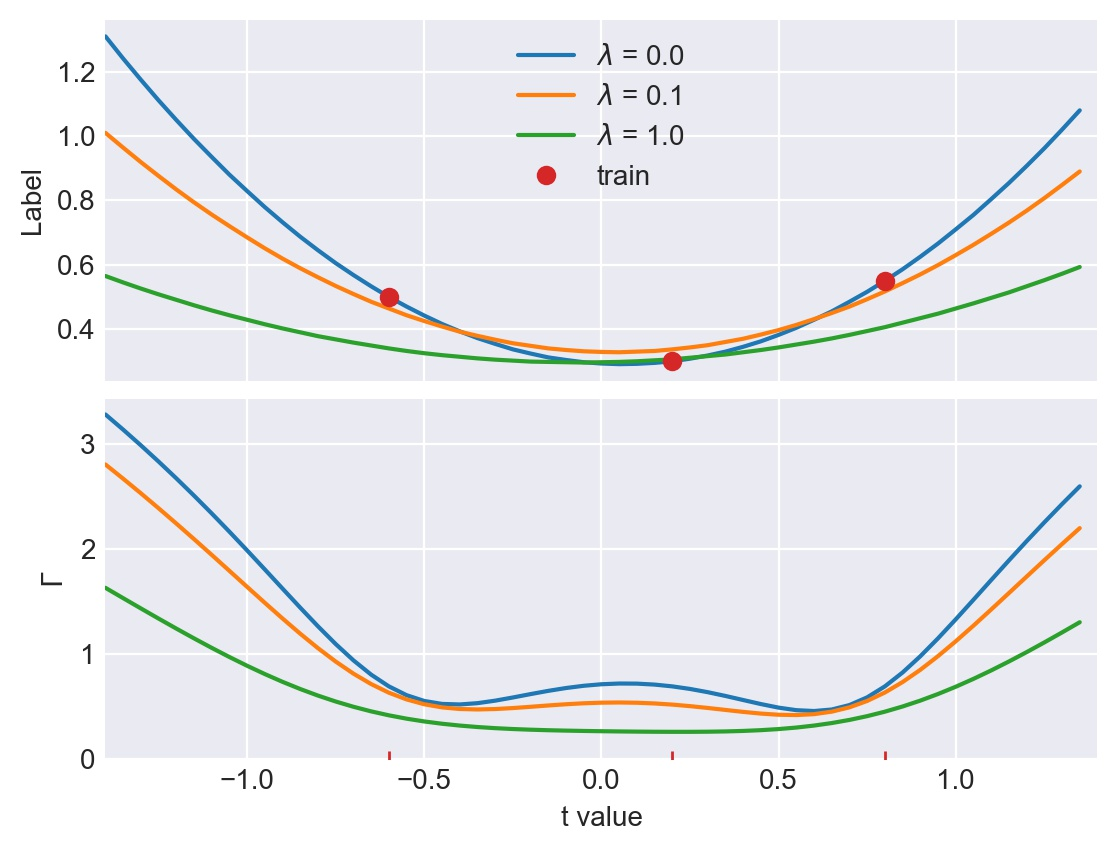
\includegraphics[width=\linewidth]{least_squares_with_regularization.jpg}
    \caption{\textbf{Least squares predictor with variety of regularization terms.} (Top) The least squares estimator fitted to the training data (in red) with different values of regularization term. (Bottom) The regret of the pNML learner from (\ref{eq:regret}) on the interval [-1,1]. The training data are marked in red on the x axis.}
    \label{fig:least_squares_with_reg}
\end{figure}

Next, we simulate the case of fitting polynomials with different degrees. 
Again, we generated 10 random points in the interval $[-1, 1]$.
The matrix $X$ is now:
\begin{equation}
X = 
\begin{bmatrix}
1 & 1 & 1 & \hdots & 1\\
t_0 & t_1 & t_2 & \hdots & t_{9}\\
\vdots &  \vdots &       & \vdots  \\
t_0^{\textit{Poly Deg}} & t_1^{\textit{Poly Deg}} & t_2^{\textit{Poly Deg}}  & \hdots & t_{9}^{\textit{Poly Deg}}
\end{bmatrix}.
\end{equation}
Figure \ref{fig:least_squares_with_poly} (top) shows the predicted label for every $t$ value in $[-1,1]$ for the different polynomial degrees. 
To avoid singularities we used the regularized version with $\lambda=10^{-4}$. 
The training set is shown by red dots in the figure. 
Note that for a polynomial of degree ten, the number of parameters is greater than the size of the training set. 
Nevertheless, the prediction accuracy near the training samples is similar to that of a degree three polynomial.
Figure \ref{fig:least_squares_with_poly} (bottom) shows the regret (or learnability) of the three pNML learners corresponding to model classes of polynomials with the various degrees. 
All the learners have regret values that are small near the training samples and large as $t$ drifts away from these samples.


\begin{figure}[tb]
    \centering
    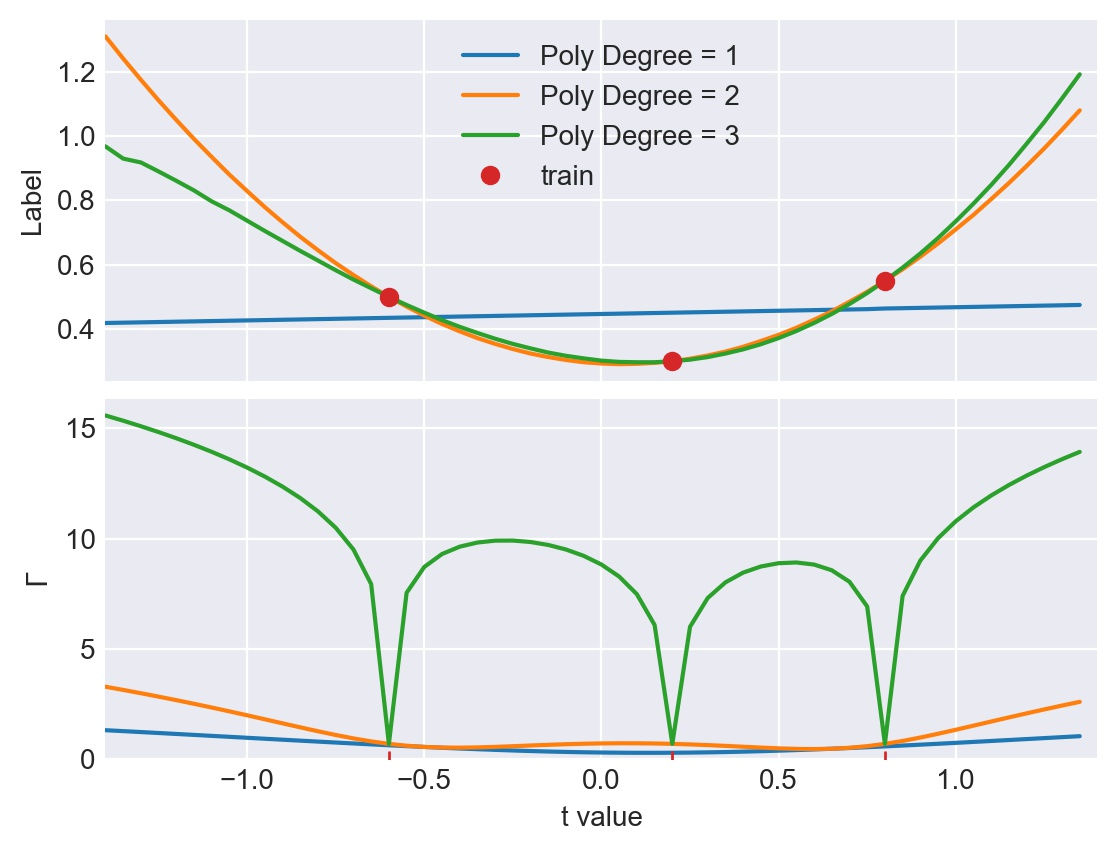
\includegraphics[width=\linewidth]{least_squares_with_poly_degree.jpg}
    \caption{\textbf{Least squares predictor with different polynomial degree.} (Top) pNML least squares predictions with different polynomial degrees. (Bottom) The regret of the pNML learners from (\ref{eq:regret}) on the interval [-1,1]. The training data t values are marked in red on the x axis.}
    \label{fig:least_squares_with_poly}
\end{figure}


\section{Conclusions} \label{sec:conclusion}

In this paper, we provided an explicit analytical solution of the pNML universal learning scheme and its learnability measure for the linear regression hypothesis class. 
Interestingly, the predicted universal pNML assignment is Gaussian with a mean that is equal to that of the ERM, but with a variance that increases by a factor $K$ whose logarithm is the learnability measure $\Gamma$.
Analyzing $\Gamma$ we can observe the ``learnability space'' for this problem. 
Specifically, if a test sample mostly lies in the subspace spanned by the eigenvectors associated with large eigenvalues of the empirical correlation matrix then the learner can generalize well, even in an over-parameterized case where the regression dimension is larger than the number of training samples.
Finally, we provided a simulation of the pNML least squares prediction for polynomial interpolation.

This work suggests a number of potential directions for future work, some are already explored in an accompanying paper \cite{pNML_neural_networks}. 
We conjecture that as in linear regression other ``over-parameterized'' model classes are learnable at least locally, that can be inferred from the pNML solution. 
This notion is indeed corroborated by the findings in \cite{pNML_neural_networks}.



%%%%%%
%% To balance the columns at the last page of the paper use this
%% command:
%%
%\enlargethispage{-1.2cm} 
%%
%% If the balancing should occur in the middle of the references, use
%% the following trigger:
%%
% \IEEEtriggeratref{3}
%%
%% which triggers a \newpage (i.e., new column) just before the given
%% reference number. Note that you need to adapt this if you modify
%% the paper.  The "triggered" command can be changed if desired:
%%
%\IEEEtriggercmd{\enlargethispage{-20cm}}
%%
%%%%%%


%%%%%%
%% References:
%% We recommend the usage of BibTeX:
%%
%\bibliographystyle{IEEEtran}
%\bibliography{definitions,bibliofile}
%%
%% where we here have assume the existence of the files
%% definitions.bib and bibliofile.bib.
%% BibTeX documentation can be obtained at:
%% http://www.ctan.org/tex-archive/biblio/bibtex/contrib/doc/
%%%%%%


%% Or you use manual references (pay attention to consistency and the
%% formatting style!):
\bibliographystyle{IEEEtran}
\bibliography{refrences}


\end{document}


%%%%%%
%% Some comments about useful packages
%% (extract from bare_conf.tex by Michael Shell)
%%

% *** MISC UTILITY PACKAGES ***
%
%\usepackage{ifpdf}
% Heiko Oberdiek's ifpdf.sty is very useful if you need conditional
% compilation based on whether the output is pdf or dvi.
% usage:
% \ifpdf
%   % pdf code
% \else
%   % dvi code
% \fi
% The latest version of ifpdf.sty can be obtained from:
% http://www.ctan.org/pkg/ifpdf
% Also, note that IEEEtran.cls V1.7 and later provides a builtin
% \ifCLASSINFOpdf conditional that works the same way.
% When switching from latex to pdflatex and vice-versa, the compiler may
% have to be run twice to clear warning/error messages.


% *** CITATION PACKAGES ***
%
%\usepackage{cite}
% cite.sty was written by Donald Arseneau
% V1.6 and later of IEEEtran pre-defines the format of the cite.sty package
% \cite{} output to follow that of the IEEE. Loading the cite package will
% result in citation numbers being automatically sorted and properly
% "compressed/ranged". e.g., [1], [9], [2], [7], [5], [6] without using
% cite.sty will become [1], [2], [5]--[7], [9] using cite.sty. cite.sty's
% \cite will automatically add leading space, if needed. Use cite.sty's
% noadjust option (cite.sty V3.8 and later) if you want to turn this off
% such as if a citation ever needs to be enclosed in parenthesis.
% cite.sty is already installed on most LaTeX systems. Be sure and use
% version 5.0 (2009-03-20) and later if using hyperref.sty.
% The latest version can be obtained at:
% http://www.ctan.org/pkg/cite
% The documentation is contained in the cite.sty file itself.


% *** GRAPHICS RELATED PACKAGES ***
%
\ifCLASSINFOpdf
  % \usepackage[pdftex]{graphicx}
  % declare the path(s) where your graphic files are
  % \graphicspath{{../pdf/}{../jpeg/}}
  % and their extensions so you won't have to specify these with
  % every instance of \includegraphics
  % \DeclareGraphicsExtensions{.pdf,.jpeg,.png}
\else
  % or other class option (dvipsone, dvipdf, if not using dvips). graphicx
  % will default to the driver specified in the system graphics.cfg if no
  % driver is specified.
  % \usepackage[dvips]{graphicx}
  % declare the path(s) where your graphic files are
  % \graphicspath{{../eps/}}
  % and their extensions so you won't have to specify these with
  % every instance of \includegraphics
  % \DeclareGraphicsExtensions{.eps}
\fi
% graphicx was written by David Carlisle and Sebastian Rahtz. It is
% required if you want graphics, photos, etc. graphicx.sty is already
% installed on most LaTeX systems. The latest version and documentation
% can be obtained at: 
% http://www.ctan.org/pkg/graphicx
% Another good source of documentation is "Using Imported Graphics in
% LaTeX2e" by Keith Reckdahl which can be found at:
% http://www.ctan.org/pkg/epslatex
%
% latex, and pdflatex in dvi mode, support graphics in encapsulated
% postscript (.eps) format. pdflatex in pdf mode supports graphics
% in .pdf, .jpeg, .png and .mps (metapost) formats. Users should ensure
% that all non-photo figures use a vector format (.eps, .pdf, .mps) and
% not a bitmapped formats (.jpeg, .png). The IEEE frowns on bitmapped formats
% which can result in "jaggedy"/blurry rendering of lines and letters as
% well as large increases in file sizes.
%
% You can find documentation about the pdfTeX application at:
% http://www.tug.org/applications/pdftex


% *** MATH PACKAGES ***
%
%\usepackage{amsmath}
% A popular package from the American Mathematical Society that provides
% many useful and powerful commands for dealing with mathematics.
%
% Note that the amsmath package sets \interdisplaylinepenalty to 10000
% thus preventing page breaks from occurring within multiline equations. Use:
%\interdisplaylinepenalty=2500
% after loading amsmath to restore such page breaks as IEEEtran.cls normally
% does. amsmath.sty is already installed on most LaTeX systems. The latest
% version and documentation can be obtained at:
% http://www.ctan.org/pkg/amsmath


% *** SPECIALIZED LIST PACKAGES ***
%
%\usepackage{algorithmic}
% algorithmic.sty was written by Peter Williams and Rogerio Brito.
% This package provides an algorithmic environment fo describing algorithms.
% You can use the algorithmic environment in-text or within a figure
% environment to provide for a floating algorithm. Do NOT use the algorithm
% floating environment provided by algorithm.sty (by the same authors) or
% algorithm2e.sty (by Christophe Fiorio) as the IEEE does not use dedicated
% algorithm float types and packages that provide these will not provide
% correct IEEE style captions. The latest version and documentation of
% algorithmic.sty can be obtained at:
% http://www.ctan.org/pkg/algorithms
% Also of interest may be the (relatively newer and more customizable)
% algorithmicx.sty package by Szasz Janos:
% http://www.ctan.org/pkg/algorithmicx


% *** ALIGNMENT PACKAGES ***
%
%\usepackage{array}
% Frank Mittelbach's and David Carlisle's array.sty patches and improves
% the standard LaTeX2e array and tabular environments to provide better
% appearance and additional user controls. As the default LaTeX2e table
% generation code is lacking to the point of almost being broken with
% respect to the quality of the end results, all users are strongly
% advised to use an enhanced (at the very least that provided by array.sty)
% set of table tools. array.sty is already installed on most systems. The
% latest version and documentation can be obtained at:
% http://www.ctan.org/pkg/array

% IEEEtran contains the IEEEeqnarray family of commands that can be used to
% generate multiline equations as well as matrices, tables, etc., of high
% quality.


% *** SUBFIGURE PACKAGES ***
%\ifCLASSOPTIONcompsoc
%  \usepackage[caption=false,font=normalsize,labelfont=sf,textfont=sf]{subfig}
%\else
%  \usepackage[caption=false,font=footnotesize]{subfig}
%\fi
% subfig.sty, written by Steven Douglas Cochran, is the modern replacement
% for subfigure.sty, the latter of which is no longer maintained and is
% incompatible with some LaTeX packages including fixltx2e. However,
% subfig.sty requires and automatically loads Axel Sommerfeldt's caption.sty
% which will override IEEEtran.cls' handling of captions and this will result
% in non-IEEE style figure/table captions. To prevent this problem, be sure
% and invoke subfig.sty's "caption=false" package option (available since
% subfig.sty version 1.3, 2005/06/28) as this is will preserve IEEEtran.cls
% handling of captions.
% Note that the Computer Society format requires a larger sans serif font
% than the serif footnote size font used in traditional IEEE formatting
% and thus the need to invoke different subfig.sty package options depending
% on whether compsoc mode has been enabled.
%
% The latest version and documentation of subfig.sty can be obtained at:
% http://www.ctan.org/pkg/subfig


% *** FLOAT PACKAGES ***
%
%\usepackage{fixltx2e}
% fixltx2e, the successor to the earlier fix2col.sty, was written by
% Frank Mittelbach and David Carlisle. This package corrects a few problems
% in the LaTeX2e kernel, the most notable of which is that in current
% LaTeX2e releases, the ordering of single and double column floats is not
% guaranteed to be preserved. Thus, an unpatched LaTeX2e can allow a
% single column figure to be placed prior to an earlier double column
% figure.
% Be aware that LaTeX2e kernels dated 2015 and later have fixltx2e.sty's
% corrections already built into the system in which case a warning will
% be issued if an attempt is made to load fixltx2e.sty as it is no longer
% needed.
% The latest version and documentation can be found at:
% http://www.ctan.org/pkg/fixltx2e


%\usepackage{stfloats}
% stfloats.sty was written by Sigitas Tolusis. This package gives LaTeX2e
% the ability to do double column floats at the bottom of the page as well
% as the top. (e.g., "\begin{figure*}[!b]" is not normally possible in
% LaTeX2e). It also provides a command:
%\fnbelowfloat
% to enable the placement of footnotes below bottom floats (the standard
% LaTeX2e kernel puts them above bottom floats). This is an invasive package
% which rewrites many portions of the LaTeX2e float routines. It may not work
% with other packages that modify the LaTeX2e float routines. The latest
% version and documentation can be obtained at:
% http://www.ctan.org/pkg/stfloats
% Do not use the stfloats baselinefloat ability as the IEEE does not allow
% \baselineskip to stretch. Authors submitting work to the IEEE should note
% that the IEEE rarely uses double column equations and that authors should try
% to avoid such use. Do not be tempted to use the cuted.sty or midfloat.sty
% packages (also by Sigitas Tolusis) as the IEEE does not format its papers in
% such ways.
% Do not attempt to use stfloats with fixltx2e as they are incompatible.
% Instead, use Morten Hogholm'a dblfloatfix which combines the features
% of both fixltx2e and stfloats:
%
% \usepackage{dblfloatfix}
% The latest version can be found at:
% http://www.ctan.org/pkg/dblfloatfix


% *** PDF and URL PACKAGES ***
%
%\usepackage{url}
% url.sty was written by Donald Arseneau. It provides better support for
% handling and breaking URLs. url.sty is already installed on most LaTeX
% systems. The latest version and documentation can be obtained at:
% http://www.ctan.org/pkg/url
% Basically, \url{my_url_here}.



% *** Do not adjust lengths that control margins, column widths, etc. ***
% *** Do not use packages that alter fonts (such as pslatex).         ***
%%%%%%


%%% Local Variables:
%%% mode: latex
%%% TeX-master: t
%%% End:

